\chapter{Project Management}

\section{Roles and Responsibilities of Team Members}

Each team member played a vital role in the group:

\medskip
\begin{itemize}[itemsep=3mm, parsep=-1mm]
    \item Kerwin oversaw the Project Management of the group and ensured that everything is going according to plan. He also assisted in contacting vendors and setting schedules up. 
    \item Nadia was responsible for the solar collector design and sizing. She was in charge of ensuring that the collector is functional.
    \item Jessica oversaw component matching and contacting sponsors about the component matching. 
    \item Charuka was the assembly lead. He was present during all assembly steps and oversaw much of the frame design as well.
    \item Dhruvi was in charge of the control and data acquisition system. 
    \item Edwin was the testing lead and also oversaw the condenser design.
\end{itemize}

\section{Project Schedule and Deliverables}
The major milestones that the team has completed is listed in the Table below. Please also see the Gantt Chart (Appendix B) for further detail.
\begin{table}[H]
\centering
\caption{Project Milestones}
\rowcolors{2}{gray!20}{white}
\begin{tabular}{|P{75mm}|P{75mm}|}
    \hline
    \rowcolor{orangeRed}
    Milestone & Scheduled Completion Date \\
    \hline
    First Iteration of Collector Design         & 15-Nov-21 \\
    Final Design with all Compatible Components & 01-Dec-21  \\
    Complete Bill of Materials                  & 21-Jan-22 \\
    Order all Components                        & 01-Mar-21 \\
    Prototype Assembled                         & 04-Apr-22  \\
    \hline
\end{tabular}
\end{table}


\section{Use of Project Resources and Contact Hours}
For this project, biweekly meetings with the sponsor and meetings with the faculty advisor were scheduled as needed. The team also met with advisors from Klass Mechanical for advice on a regular basis as well.

\section{Cost Overview}
A budget of \$10,000 was provided to the team to construct the prototype. The team had to be conscious of how much each component costs to remain under budget. Figure () shows a brief cost breakdown of the components that comprises the prototype.

\medskip
\begin{figure}[H]
    \centering
    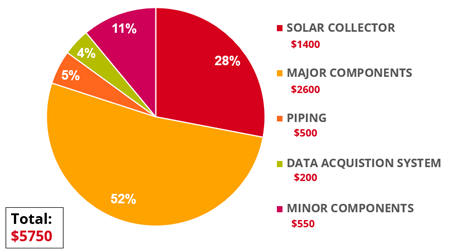
\includegraphics[width=10cm]{images/cost_breakdown.png}
    \caption{Cost Breakdown of Prototype}
\end{figure}

\medskip
Costs that are not accounted for are the costs of the expansion valve, compressor, pressure transducer and the insulation as they were provided by a sponsor.